\subsection{OR問題を学習させた際の誤差収束度合いについて}
\subsubsection{実験結果}
NNでは重みを更新する毎に誤差が減るように学習を行うが、
その学習の様子は初期の重みをどのように設定したか、
学習に用いたパラメータをどのように設定したか、
といった対象問題以外の要素に影響して学習の様子が変化する。
シード値を変えた際の学習収束回数を表\ref{table:level1}に示す。
シード値を10回変更して学習させた際の重みを更新する様子を図
\ref{fig:level1-1}に、
その平均をプロットした平均推移値を図\ref{fig:level1-2}に示す。
なお、平均値を求める際には10回分の実行データを加工して統合,平均値を算出した。
具体的には一行ごとに実行データから抜き取り,10回分を加算し,加算回数で割って求めている。
(src/bp\_mo配下のintegration.shを参照)

\begin{table}[htb]
 \begin{center}
  \caption{OR問題の学習に要した回数}
  \label{table:level1}
  \begin{tabular}[htb]{r|l} \hline
   シード値 & 収束した回数 \\ \hline \hline
   1000 & 96 \\ \hline
   2000 & 90 \\ \hline
   3000 & 111 \\ \hline
   4000 & 109 \\ \hline
   5000 & 93 \\ \hline
   6000 & 99 \\ \hline
   7000 & 100 \\ \hline
   8000 & 114 \\ \hline
   9000 & 113 \\ \hline
   10000 & 94 \\ \hline \hline
   10試行の平均値 & 101.9 \\ \hline
  \end{tabular}
 \end{center}
\end{table}


\begin{figure}[h]
 \begin{center}
  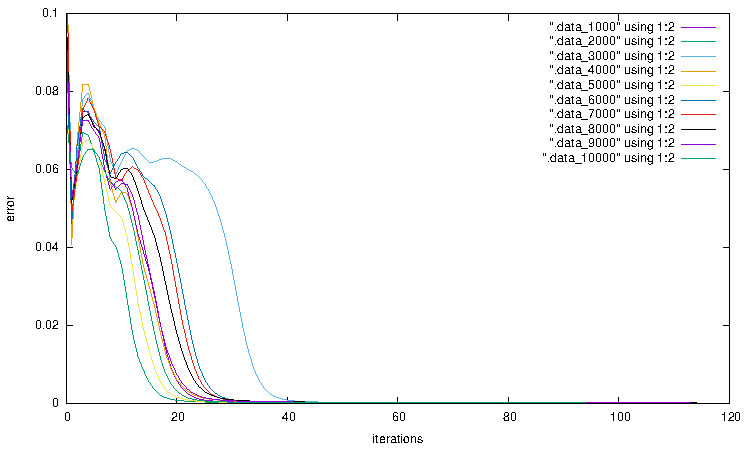
\includegraphics[width=10.0cm]{figs/level1/iterations_vs_error.pdf}
  \caption{重みを更新する様子}
  \label{fig:level1-1}
 \end{center}
\end{figure}

\begin{figure}[h]
 \begin{center}
  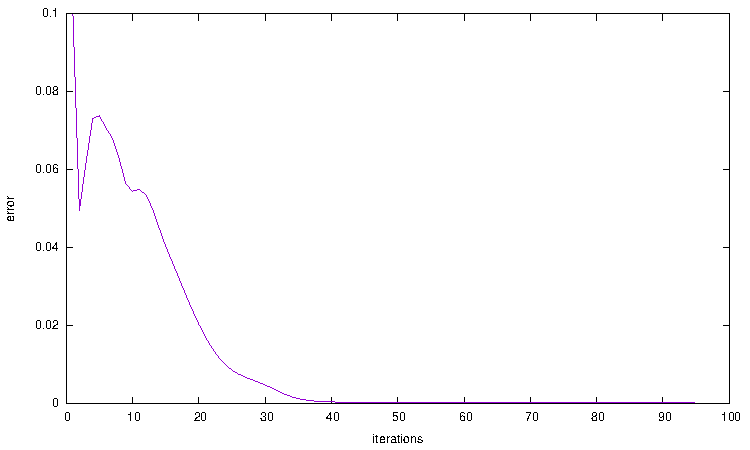
\includegraphics[width=10.0cm]{figs/level1/ave.pdf}
  \caption{重みを更新する様子(平均値)}
  \label{fig:level1-2}
 \end{center}
\end{figure}


\subsubsection{考察}
実験よりわかったことを以下に箇条書きする.\\
\begin{itemize}
	\item すべてFINISH2で終わったため,誤差が最小誤差より小さくなっている.
	\item 実験が収束したのは100前後で,seed値をこれ以上大きくしてみても同じように100前後で収束すると推測する.
	\item 学習曲線は,errorが0.05くらいまで急激に下がり,その後若干上がり,そのあと最小誤差へと遷移している.
\end{itemize}


